\documentclass[12pt]{article}
 \usepackage[margin=1in]{geometry} 
\usepackage{amsmath,amsthm,amssymb,amsfonts}
 \usepackage{graphicx}
\usepackage{caption}
\usepackage{subfigure}

\newcommand{\N}{\mathbb{N}}
\newcommand{\Z}{\mathbb{Z}}
 
\newenvironment{problem}[2][Problem]{\begin{trivlist}
\item[\hskip \labelsep {\bfseries #1}\hskip \labelsep {\bfseries #2.}]}{\end{trivlist}}
%If you want to title your bold things something different just make another thing exactly like this but replace "problem" with the name of the thing you want, like theorem or lemma or whatever
 
\begin{document}
 
%\renewcommand{\qedsymbol}{\filledbox}
%Good resources for looking up how to do stuff:
%Binary operators: http://www.access2science.com/latex/Binary.html
%General help: http://en.wikibooks.org/wiki/LaTeX/Mathematics
%Or just google stuff
 
\title{Project 2B Report}
\author{Yutong Han 705025619 \\
		\\
		\\
		\\
		}
\maketitle
 
\section{Time Series Plot}
The Figure.\ref{fig:1} shows the time series plot( by day) of positive and negative sentiment.

\begin{figure}[!h]
     \begin{center}
                  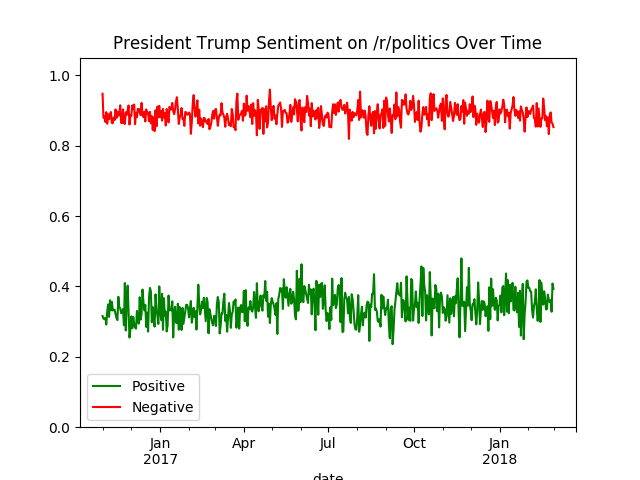
\includegraphics[width=0.8\textwidth]{../plots/part1.png}
    \end{center}
    \caption{%
       Time Series Plot 
     }%sl
   \label{fig:1}
\end{figure}



\section{Positive and Negative Sentiment of US State}
The Figure.\ref{fig:2} and Figure.\ref{fig:3} shows the time series plot( by day) of positive and negative sentiment.

\begin{figure}[!h]
      \centering
    \begin{subfigure}
        \centering
        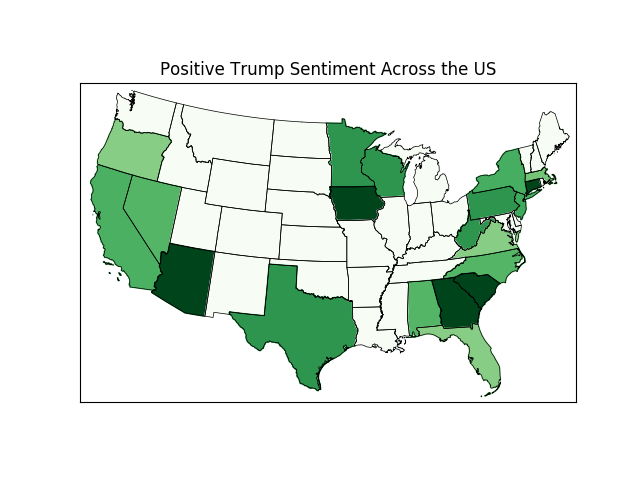
\includegraphics[width=0.7\textwidth]{../plots/part2_pos.png}
        \caption{Positive Sentiment over US States}
        \label{fig:2}
    \end{subfigure}%
    \vspace{1em}
    \begin{subfigure}
       \centering
        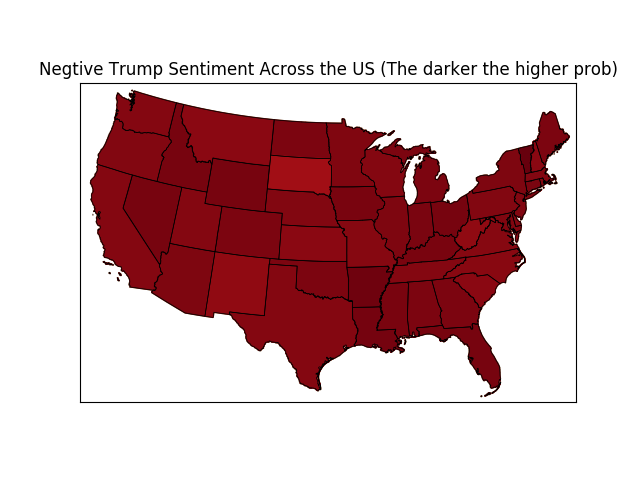
\includegraphics[width=0.7\textwidth]{../plots/part2_neg.png}
        \caption{Negative Sentiment over US States}
        \label{fig:3}
    \end{subfigure}
\end{figure}


\newpage 
\section{Sentiment Difference of US State}
The Figure.\ref{fig:4} shows the different of positive and negative sentiment across the US States.

\begin{figure}[!h]
     \begin{center}
                  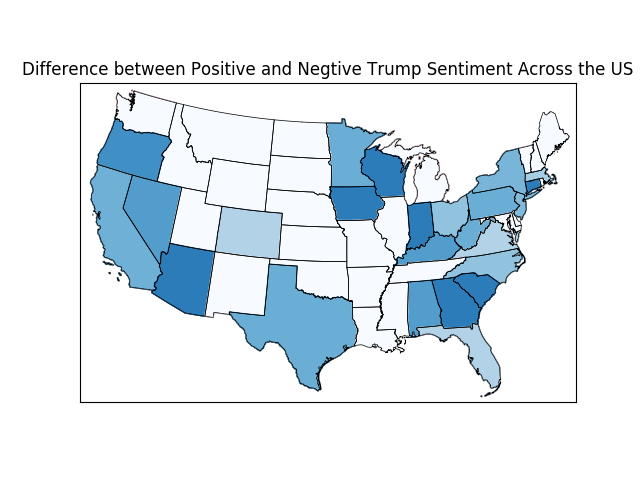
\includegraphics[width=0.8\textwidth]{../plots/part3.png}
    \end{center}
    \caption{%
       Difference between the positive and negative sentiment across US States.
     }%sl
     \label {fig:4}
 \end{figure}
 
 \section{Top 10 positive stories}
 \section{Create TWO scatterplots where the X axis is the submission score,}
 \section {Produce the ROC curves}
\section {summarizing your finding}
\section {Question 1}
Take a look at $labeled\_data.csv$ Write the functional dependencies implied by the data.

\textbf {Answer:} The $Input\_id$ is the primary key of the scheme. So the $Input\_id \to labeldem$,  $Input\_id \to labelgop$, $Input\_id \to labeldjt$ and their combinations can be implied. 
\section {Question 2}
Take a look at the schema for the comments dataframe. Forget BCNF and 3NF. Does the data frame look normalized? In other words, is the data frame free of redundancies that might affect insert/update integrity? If not, how would we decompose it? Why do you believe the collector of the data stored it in this way?

\textbf{Answer:} It does not look normalized. In the $subreddit\_id$ and $subreddit$ part, it seems that the  $subreddit\_id \to subreddit$. So the $subreddit$ may store repeatedly. So it can be decomposed into two scheme with the $subreddit$ be the key of other scheme. Since this database may contains about the posts about the politics, the subreddit is just the \textit{/r/politics}


\section {Question 3}
 







\end{document}